\chapter{MELON Implementation}\label{chapter:implementation}

\section{Architecture}

\begin{figure}
\centering
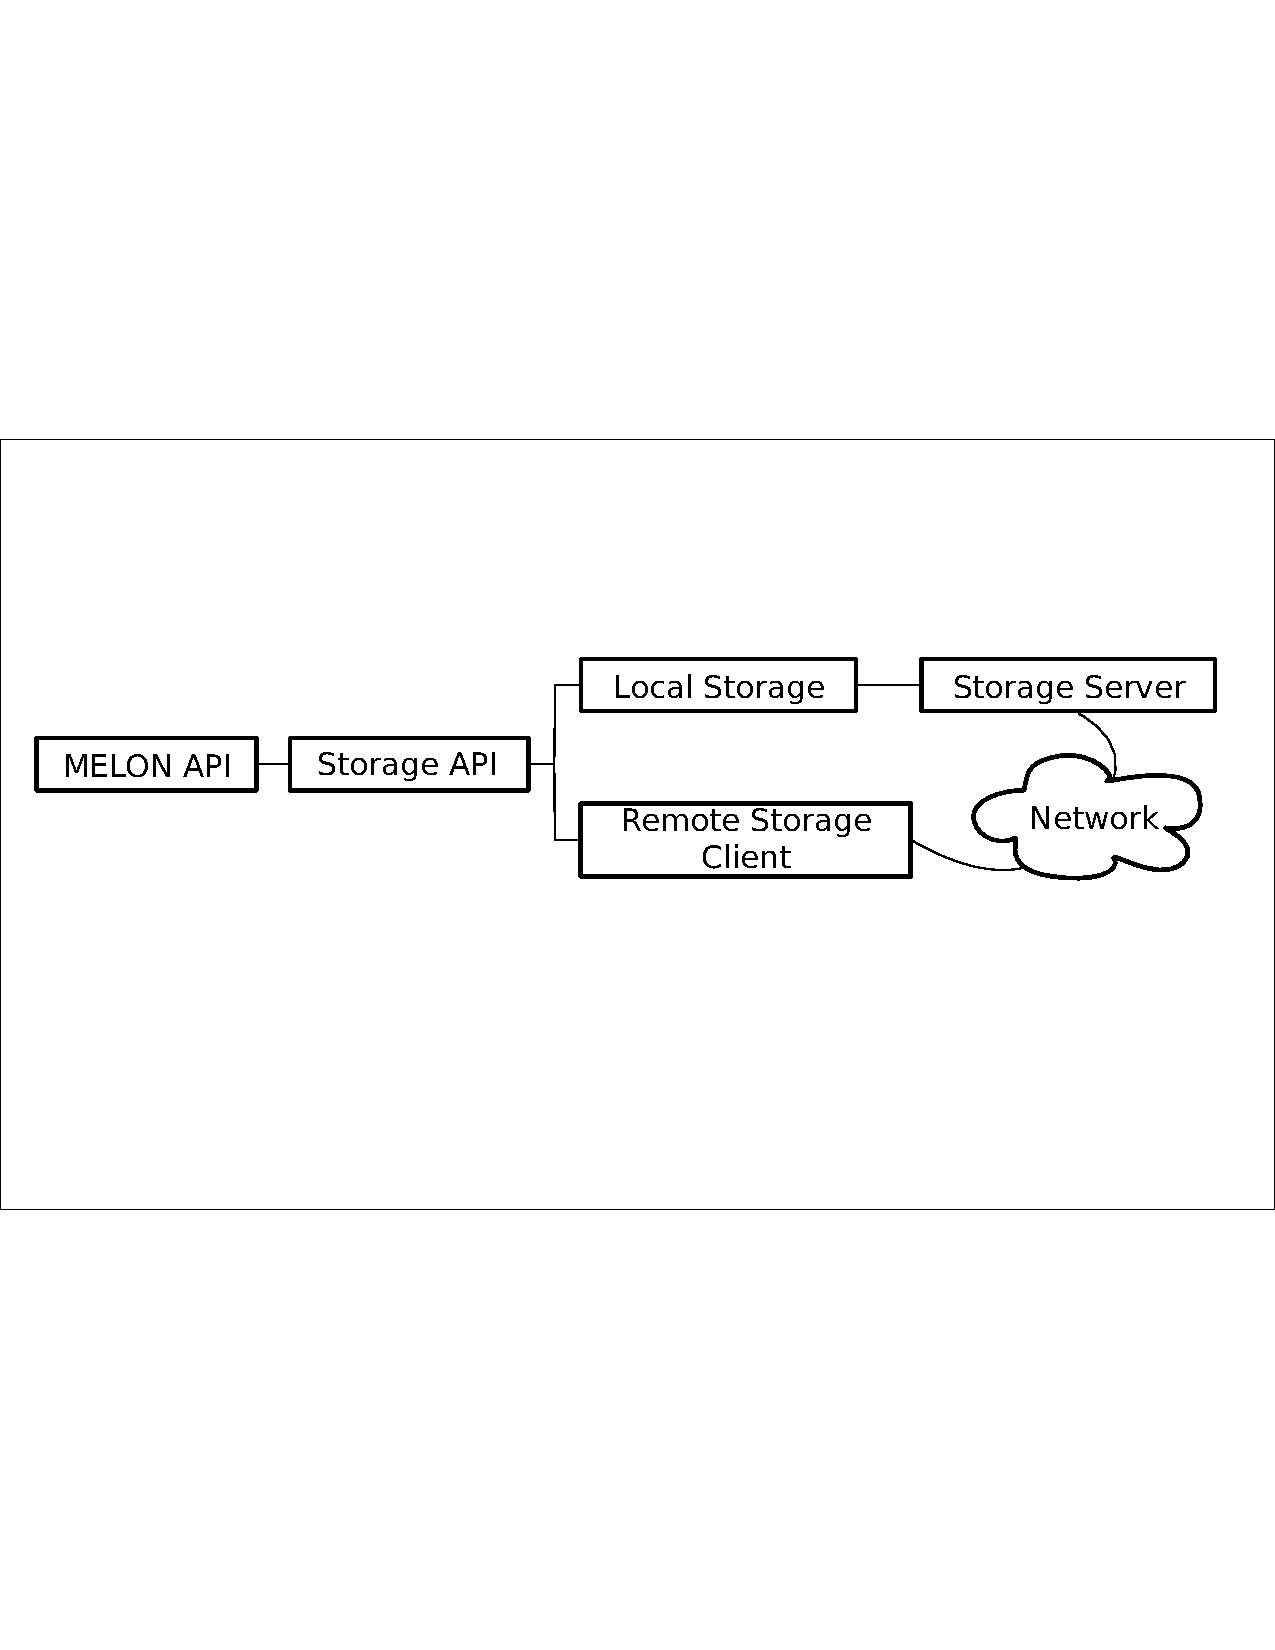
\includegraphics[scale = .70, clip, trim = 10px 280px 10px 250px]{figures/paradigm_arch.pdf}
\caption{Paradigm Architecture}
\label{fig:architecture}
\end{figure}

We developed a prototype implementation of MELON to validate our design and obtain empirical performance data. The architecture illustrated in Figure \ref{fig:architecture} is split into five parts. The MELON API is the only interface exposed to the application and provides the six operations described above. The MELON API interacts with the distributed message storage through the storage API, which provides the same interface for both local and remote storage. The storage server proves a network interface to a local storage space and accepts connections made through the remote storage stub.

Local storage is implemented simply as two dynamic arrays, one for write/read messages and the other for \textbf{store}/\textbf{take} messages. For atomic updates, the \textbf{write}/\textbf{read} array uses a readers/writer lock to allow multiple \textbf{read} operations to access the array in parallel, but locks the array for \textbf{write} operations. The \textbf{store}/\textbf{take} array does not permit concurrent operations, since both \textbf{store} and \textbf{take} modify the store. The two arrays may be accessed and modified independently.

\section{Networking}

Network communication is handled using ZeroMQ\cite{hintjens2013zeromq}, a high performance high level networking library. For the prototype, the network communication was intentionally kept simple. For example, a \textbf{read} request queries remote hosts in a random order and stops when a matching result is returned. While it is possible to improve this using multicast, it would greatly complicate the implementation by requiring the client to handle multiple asynchronous responses, choose between them, request the actual matching message, and then handle failure scenarios if the matching message cannot be returned. Our approach was to trade off potential performance gains for simplicity.

\section{Read Message Tracking}

When a messages is stored, it is given a unique identifier [\textit{P}, \textit{M}], where \textit{P} is a globally unique integer identifier for the storing process, and \textit{M} is an integer identifier for the stored message. Each process maintains an integer ID which is incremented for each store. Messages stored from the same process with sequential \textbf{store} or \textbf{write} operations will have consecutive \textit{M} values and share the same \textit{P} value.

In order to prevent \textbf{read} from returning a message more than once in the same process, each process maintains a sparse bit set for each process from which a message has been read. The identifier [\textit{P}, \textit{M}] is condensed into a single unique integer \textit{Q} using the ``elegant pairing function''\cite{szudzikelegant} shown in Equation \ref{eq:elegantpairing}. Since the values of \textit{Q} will be consecutive integers for all consecutive values of $M < P$, it is helpful to set \textit{P} to be higher than the number of expected messages. The value \textit{Q} is then stored in a sparse bit set with a hash table using integer keys and bit field values.

 \begin{equation}
   f(M,P) = \left\{
     \begin{array}{lr}
       M^{2} + M + P & : M \geq P \\
       P^{2} + M & : M < P
     \end{array}
   \right.
   \label{eq:elegantpairing}
\end{equation}

The index \textit{i} in the sparse bit set indicates the range stored in the bit set. If \textit{w} is the number of bits for each bit set, then each bit field can store up to \textit{w} values of \textit{n}, where $w \times i \leq n < w \times (i + 1)$. A message with ID \textit{n} will be stored in index $n/w$ by setting the bit at $n \bmod w$ in the bit field to \texttt{1}.

If the index value is of size \textit{l} bits and the bit field contains \textit{w} bits, then the cost for storing a single value is $l + w$. For storing a set of consecutive values of length \textit{m}, the cost is $\lfloor \frac{m \times l}{w} \rfloor + m$ bits. In other words, the total cost is one bit per message, plus the cost of one index per \textit{w} messages.

\begin{table}
\centering
\caption{Sparse bit set example}
\begin{tabular}{|c|c|} \hline
Index & Bit Field \\ \hline
0 & 01100001 \\ \hline
4 & 00010000 \\ \hline
15 & 10100100 \\ \hline
\end{tabular}
\label{fig:bitset}
\end{table}

Consecutive messages (from any starting value) are the best-case scenario for sparse bit sets. In the worst case, the message IDs differ by at least \textit{w}, causing each message to incur a $l + w$ cost for storage and a total cost of $m \times (l + w)$ bits.

Determining if a message [\textit{P}, \textit{M}] is in the set is accomplished by first computing \textit{Q}. If there is no key at index $Q/w$, the message has not been read. Otherwise, retrieve the bit field \textit{b} at index $M / w$. If $b \wedge 2^{M \bmod w} \neq 0$ then the message has been read, otherwise the message is unread.

\section{Message Replication}

Message replication may be implemented as an additional feature of MELON without adding any new operations. Distributing copies of messages to multiple hosts can increase message availability even in the face of network partitioning. However, only read-only messages may be replicated. Since take-only messages may only be taken once, atomic removals would need to be coordinated across all hosts with a replicated copy of the removed message. In a MANET, this is not practical and in many cases it will not be possible. A node containing a replicated message may leave the network with it and never return.

Read-only messages are intended to be read by multiple hosts and cannot be explicitly removed, making them candidates for replication. 

\section{Garbage Collection}

Storage space in MELON is explicitly bounded, which means applications can expect messages to be garbage collected from the shared message store if 

